\documentclass[../main.tex]{subfiles}
\graphicspath{{\subfix{../images/}}}
\begin{document}

Hyperbolic and parabolic trajectories present some interesting differences to their elliptic counterparts. These will be examined in this section.

\subsection{Hyperbolic Trajectory}\label{sec:Hyperbolic Orbits}

\begin{figure}[H]
    \centering
    \begin{tikzpicture}[>=latex]
        \def\ecc{1.2}
        \def\m{\fpeval{sqrt(\ecc^2-1)}}

        \draw[scale=1,domain=-2:2,smooth,variable=\t, <-<, thick] plot ({-cosh(\t)+\ecc},{-\m*sinh(\t)});
        \filldraw[] (0,0) circle (2pt);

    \end{tikzpicture}
    \caption{A hyperbolic trajectory}\label{fig:Hyperbolic Trajectory}
\end{figure}

An orbit is described by Equation \eqref{Polar Final}. However, for the sake of analysis, this will be transformed into cartesian coordinates. Equation \eqref{Orbit Cartesian} will be rewritten so that there are no complex arguments. Recall that for hyperbolic orbits, $e>1$ and $a<0$.

\begin{align*}
    \left(\frac{x+ea}{a}\right)^2+\left(\frac{y}{a\sqrt{1-e^2}}\right)^2              & =1 \\
    \left(\frac{x+ea}{a}\right)^2+\left(\frac{y}{ai\sqrt{e^2-1}}\right)^2             & =1 \\
    \left(\frac{x+ea}{a}\right)^2+\frac{1}{i^2}\left(\frac{y}{a\sqrt{e^2-1}}\right)^2 & =1 \\
    \left(\frac{x+ea}{a}\right)^2-\left(\frac{y}{a\sqrt{e^2-1}}\right)^2              & =1 \\
\end{align*}

This trajectory can be parameterized. It can be seen that the radius in the $x$ direction is $a$, while the radius in the $y$ direction is $a\sqrt{e^2-1}$. The hyperbola is also translated $-ea$. This can be parameterized using hyperbolic sine and hyperbolic cosine. The semi-major axis will also be factored out to simplify the expression.
\begin{equation}\label{Hyperbola Parametric}
    \vv{r}(s)=a\left\langle\cosh(s)-e, \sqrt{e^2-1}\sinh(s)\right\rangle
\end{equation}

The parameter $s$ is used instead of the typical $t$ to show that this parameterization does \textit{not} describe the location of a satellite with respect to time, but instead describes the geometry of the trajectory.

Hyperbolas approach a tangent line in their end behavior. Finding the angle $\theta_\text{hyp}$ of this tangent line to the horizontal will prove useful to analysis of the hyperbola. This will be done by finding the end behavior of the derivative of the parameterization.

\begin{align*}
    \vv{r}'(s)        & =a\left\langle\sinh(s)-e, \sqrt{e^2-1}\cosh(s)\right\rangle                                                                  \\
    \theta_\text{hyp} & =\lim_{s\rightarrow\infty}\arctan\left(\frac{y}{x}\right)                                                                    \\
                      & =\lim_{s\rightarrow\infty}\arctan\left(\frac{\sqrt{e^2-1}\cosh(s)}{\sinh(s)-e}\right)                                        \\
                      & =\lim_{s\rightarrow\infty}\arctan\left(\sqrt{e^2-1}\frac{\cosh(s)}{\sinh(s)-e}\right)                                        \\
                      & =\arctan\left(\lim_{s\rightarrow\infty}\left(\sqrt{e^2-1}\frac{\cosh(s)}{\sinh(s)-e}\right)\right)                           \\
                      & =\arctan\left(\sqrt{e^2-1}\lim_{s\rightarrow\infty}\left(\frac{\cosh(s)}{\sinh(s)-e}\right)\right)                           \\
                      & =\arctan\left(\sqrt{e^2-1}\lim_{s\rightarrow\infty}\left(\frac{\frac{d}{ds}\cosh(s)}{\frac{d}{ds}(\sinh(s)-e)}\right)\right) \\
                      & =\arctan\left(\sqrt{e^2-1}\lim_{s\rightarrow\infty}\left(\frac{\sinh(s)}{\cosh(s)}\right)\right)                             \\
                      & =\arctan\left(\sqrt{e^2-1}\lim_{s\rightarrow\infty}\left(\tanh(s)\right)\right)                                              \\
                      & =\arctan\left(\sqrt{e^2-1}\right)                                                                                            \\
\end{align*}

The angle from the horizontal (that is to say, a line passing through the periapsis and the planet) to the beginning/end tangent line is
\begin{equation}\label{Hyperbolic entry/exit angle}
    \theta_\text{hyp}=\arctan\left(\sqrt{e^2-1}\right)
\end{equation}

\begin{figure}[H]
    \centering
    \begin{tikzpicture}[>=latex]
        \def\ecc{1.2}
        \def\arcRad{3}
        \def\m{\fpeval{sqrt(\ecc^2-1)}}
        \def\thtaHyp{\fpeval{atand(\m)}}

        \draw[scale=0.1,domain=-4.5:4.5,smooth,variable=\t, <-<, gray, thin] plot ({-cosh(\t)+\ecc},{-\m*sinh(\t)});
        \filldraw[] (0,0) circle (1pt);

        \draw[dashed] (0.5,0.5*\m) -- (-5,-5*\m);
        \draw[dashed] (0.5,-0.5*\m) -- (-5,5*\m);

        \draw[] (-\arcRad,0) arc (180:180+\thtaHyp:\arcRad) node[midway, right] {$\theta_\text{hyp}$};
        \draw[] (180-\thtaHyp:1.5*\arcRad) arc (180-\thtaHyp:180+\thtaHyp:1.5*\arcRad) node[midway, left] {$2\theta_\text{hyp}$};

    \end{tikzpicture}
    \caption{A hyperbolic trajectory with the tangent lines indicated}\label{Hyperbola with angles}
\end{figure}

\subsubsection{Hyperbola Eccentricity in Terms of \texorpdfstring{$\theta_\text{hyp}$}{Theta Hyperbolic}}

From equation \eqref{Hyperbolic entry/exit angle}, the eccentricity can be isolated.
\begin{align*}
    \theta_\text{hyp}       & =\arctan\left(\sqrt{e^2-1}\right) \\
    \tan(\theta_\text{hyp}) & =\sqrt{e^2-1}                     \\
    e^2-1                   & =\tan^2(\theta_\text{hyp})        \\
    e^2                     & =1+\tan^2(\theta_\text{hyp})      \\
    e^2                     & =\sec^2(\theta_\text{hyp})        \\
\end{align*}
\begin{equation}\label{Hyperbola Eccentricity}
    e=\sec(\theta_\text{hyp})
\end{equation}

\subsubsection{Hyperbola Semi-Major Axis in Terms of Periapsis}

Equations \eqref{Periapsis Radius Geometric} and \eqref{Hyperbola Eccentricity} can be combined to isolate the semi-major axis in terms of the periapsis radius.

\begin{align*}
    r_\text{pe} & =a(1-e)                       \\
    r_\text{pe} & =a(1-\sec(\theta_\text{hyp})) \\
\end{align*}
\begin{equation}\label{Hyperbola SMA}
    a=\frac{{r_\text{pe}}}{1-\sec(\theta_\text{hyp})}
\end{equation}

\bigskip\bigskip
\subsection{Parabolic Trajectories}\label{sec:Analysis of parabolic trajectories}

\begin{figure}[H]
    \centering
    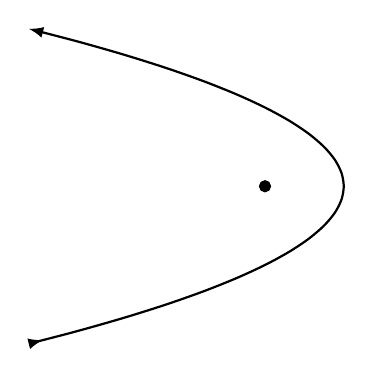
\begin{tikzpicture}[>=latex]

        \draw[scale=1,domain=-2:2,smooth,variable=\t, >->, thick] plot ({-(\t)^2+1},\t);
        \filldraw[] (0,0) circle (2pt);

    \end{tikzpicture}
    \caption{A parabolic trajectory}\label{fig:Parabolic Trajectory}
\end{figure}

The eccentricity of a parabola is, by definition, $e=1$. It is also proven in Section \ref{sec:Kepler's First Law} that when $e=1$ the orbit equation creates a parabola. For the numerator of the orbit equation $r=\frac{a(1-e^2)}{1+e\cos(\theta)}$ to be nonzero, $a$ must be infinite. The velocity in a parabolic orbit can be investigated with Equation \eqref{Vis-Viva Equation}.

\begin{align*}
    v & =\sqrt{\frac{2\mu}{r}-\frac{\mu}{a}}                                                     \\
      & =\sqrt{\frac{2\mu}{r}-\lim_{a\rightarrow\infty}\left(\frac{\mu}{a}\right)}               \\
      & =\sqrt{\frac{2\mu}{r}-\cancelto{0}{\lim_{a\rightarrow\infty}\left(\frac{\mu}{a}\right)}} \\
\end{align*}
\begin{equation}
    v_\text{parabola}=v_\text{esc}=\sqrt{\frac{2\mu}{r}}
\end{equation}

Since a parabola has a determined unique shape, there is only one parameter for it; its size. The defining parameter for a parabolic trajectory is either the periapsis $r_\text{pe}$ or the semi-latus rectum $p$, which can be related using Equation \eqref{Polar with p, e} keeping in mind that at periapsis the cosine will evaluate to 1
\begin{align*}
    r           & =\frac{p}{1+e\cos(\theta-\omega)} \\
    r_\text{pe} & =\frac{p}{1+\cos(0)}              \\
    r_\text{pe} & =\frac{p}{2}                      \\
\end{align*}
\begin{equation}
    p_\text{parabola}=2r_\text{pe,parabola}
\end{equation}

To determine the periapsis of a parabolic trajectory from a measured velocity, angular momentum must be used

\begin{align*}
    h_\text{pe}            & = h                                                   \\
    r_\text{pe}v_\text{pe} & =rv\cos(\phi)                                         \\
    r_\text{pe}            & =\frac{rv\cos(\phi)}{v_\text{pe}}                     \\
                           & =\frac{rv\cos(\phi)}{\sqrt{\frac{2\mu}{r_\text{pe}}}} \\
    r_\text{pe}^2          & =\frac{r^2v^2\cos^2(\phi)}{\frac{2\mu}{r_\text{pe}}}  \\
    r_\text{pe}^2          & =\frac{r_\text{pe}r^2v^2\cos^2(\phi)}{2\mu}           \\
\end{align*}
\begin{equation}\label{Periapsis Radius Parabola}
    r_\text{pe,parabola}=\frac{r^2v^2\cos^2(\phi)}{2\mu}
\end{equation}

\bigskip\bigskip
\subsection{Conclusion}

\bigskip
Hyperbolic orbits approach a linear trajectory with an angle of
$$\theta_\text{hyp}=\arctan\left(\sqrt{e^2-1}\right)$$

\bigskip
Because hyperbolas don't have physically meaningful apoapses, the semi-major axis and eccentricity can be defined in terms of the entry/exit angle $\theta_\text{hyp}$ and the periapsis radius $r_\text{pe}$.
$$e=\sec(\theta_\text{hyp})\qquad\qquad a=\frac{{r_\text{pe}}}{1-\sec(\theta_\text{hyp})}$$

\bigskip
Parabolic trajectories occur at exactly escape velocity, meaning that at all points
$$v=\sqrt{\frac{2\mu}{r}}$$

\bigskip
In a parabolic trajectory, the semi-latus rectum and periapsis are related by
$$p_\text{parabola}=2r_\text{pe,parabola}$$

\bigskip
From telemetry data, the periapsis radius can be found with
$$r_\text{pe,parabola}=\frac{r^2v^2\cos^2(\phi)}{2\mu}$$

\end{document}